\newcommand{\DoubleImage}{true}	%Diagramms: Two on one page?

\documentclass{beamer}

%% \usepackage[ngermanb.sty]{babel}
\usepackage[utf8]{inputenc}
\usepackage{hyperref}
\usepackage{graphicx}
\usepackage{listings}
\usepackage{ifthen}

%\usepackage[demo]{graphicx}
\usepackage[compatibility=false]{caption}
\usepackage{subcaption}

\usepackage{color}
\lstdefinestyle{customc}{
  belowcaptionskip=1\baselineskip,
  breaklines=true,
%  frame=L,
  xleftmargin=\parindent,
%  language=C,
  showstringspaces=false,
  basicstyle=\footnotesize\ttfamily,
  keywordstyle=\bfseries\color{green!40!black},
  commentstyle=\itshape\color{purple!40!black},
  identifierstyle=\color{blue},
  stringstyle=\color{orange},
}

\usetheme{Berlin}		%Szeged
\usecolortheme{dolphin}	%beaver

\setbeamercovered{transparent}
\beamertemplatenavigationsymbolsempty
%\setbeamertemplate{footline}[frame number]

%% Variablen - anpassen!
\newcommand{\theauthor}{6c8e27db312c23968fc6c6f7bb20dea0}

\newcommand{\thedate}{January 11, 2016}

\newboolean{DoublePaged} 
\setboolean{DoublePaged}{\DoubleImage} 


\title{Cache}
\subtitle{Exercise 2}
\author{\theauthor}
%\institute[LRR TUM]{LRR, I10\\ TU München}
\date{\thedate}

\begin{document}

\frame{
	\titlepage
}


\begin{frame}[fragile]
  \frametitle{cache\_flush}
  
\begin{lstlisting}[language=c,style=customc]
static inline void flush_cache(volatile void *ptr, size_t len){
for(size_t i = 0; i < len; i++, ptr++)
asm volatile ("clflush (%0)" : : "r"(ptr));
}
\end{lstlisting}
  
\end{frame}


\begin{frame}[fragile]
	\frametitle{Cache Line Length: C2D t9400}
	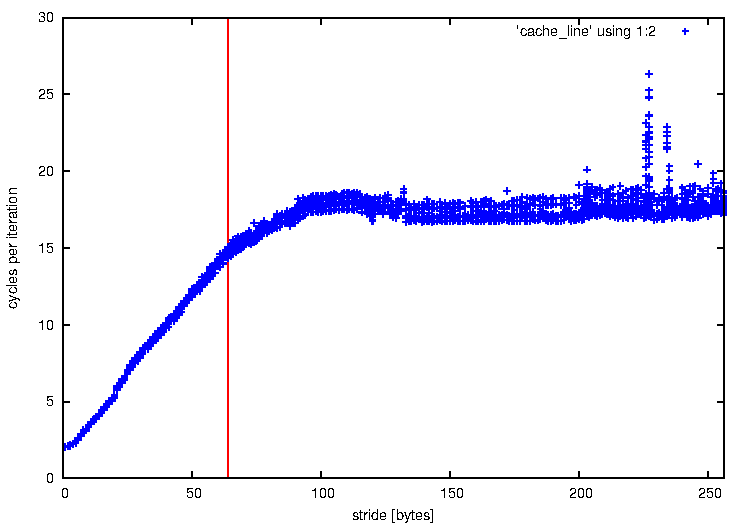
\includegraphics[width=0.9\textwidth]{../c2d_t9400/cache_line.pdf}
\end{frame}

\begin{frame}[fragile]
	\frametitle{Cache Size Small: C2D t9400}
	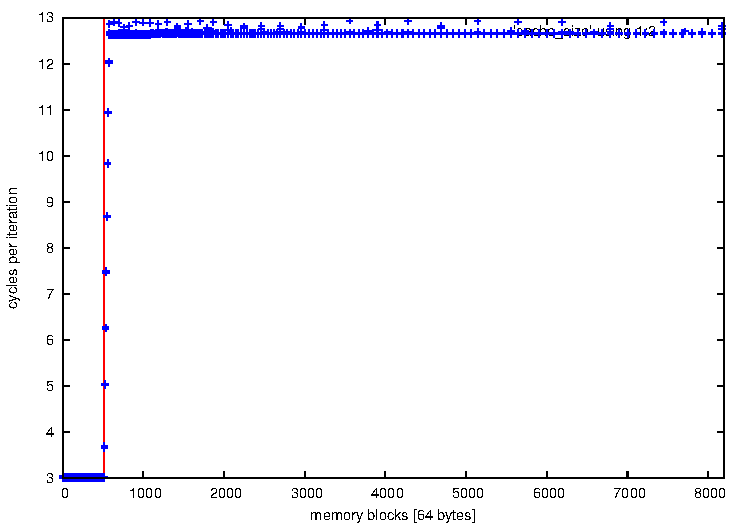
\includegraphics[width=0.9\textwidth]{../c2d_t9400/cache_size_small.pdf}
\end{frame}

\begin{frame}[fragile]
	\frametitle{Cache Size: C2D t9400}
	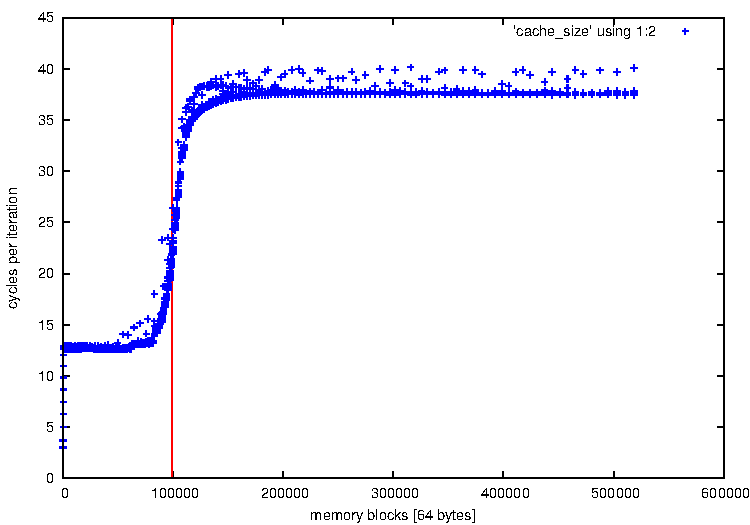
\includegraphics[width=0.9\textwidth]{../c2d_t9400/cache_size_all.pdf}
\end{frame}


\begin{frame}[fragile]
	\frametitle{Cache Line Length: Xeon e3 1230v3}
	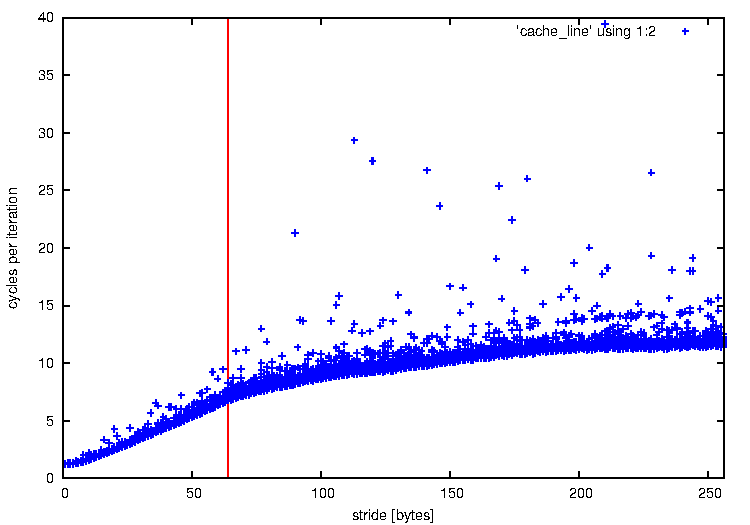
\includegraphics[width=0.9\textwidth]{../xeon_e3_1230v3/cache_line.pdf}
\end{frame}

\begin{frame}[fragile]
	\frametitle{Cache Size Small: Xeon e3 1230v3}
	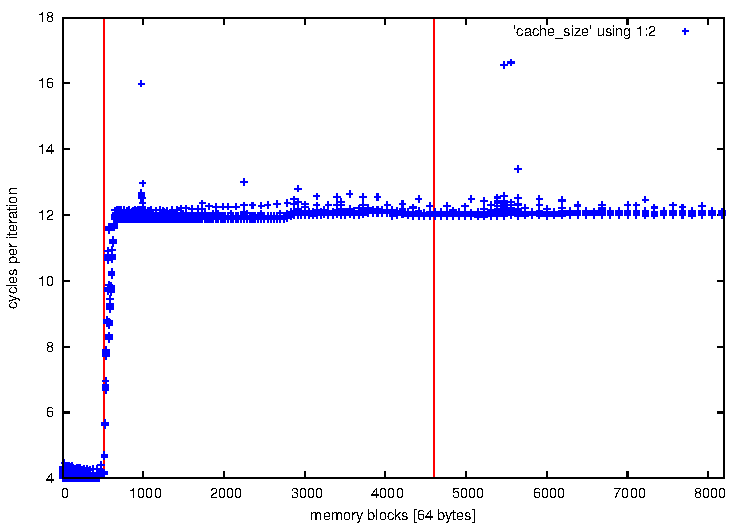
\includegraphics[width=0.9\textwidth]{../xeon_e3_1230v3/cache_size_small.pdf}
\end{frame}

\begin{frame}[fragile]
	\frametitle{Cache Size: Xeon e3 1230v3}
	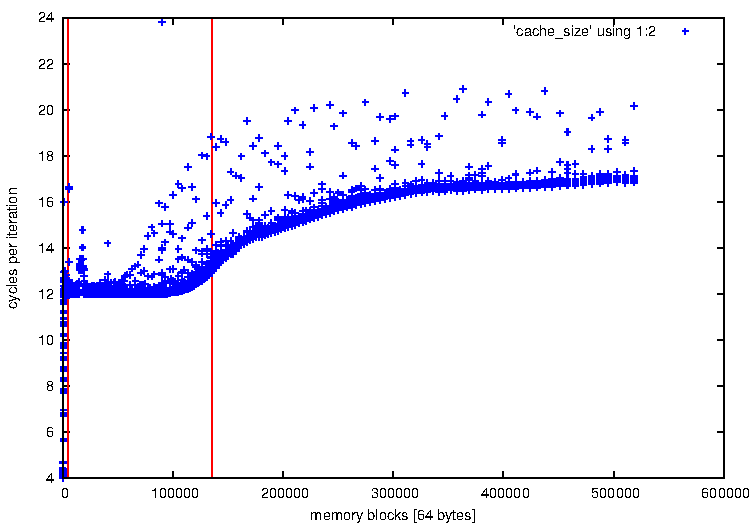
\includegraphics[width=0.9\textwidth]{../xeon_e3_1230v3/cache_size_all.pdf}
\end{frame}

\end{document}
